\chapter{Servidor}
\section{Tareas programas en el servidor}
\subsection{Actualización automática de los datos}
Una vez tenemos un primer conjunto de datos es posible que alguno de ellos cambie con el tiempo por lo que debemos de, periódicamente, lanzar un proceso que compruebe si los datos almacenados están actualizados. Para realizar esta tarea crearemos en el servidor que mantiene la aplicación una serie de tareas que se ejecutarán de manera automática.

Esta acción es de especial relevancia en el caso de las noticias, ya que a partir de nuevas noticias podremos intentar los sistemas de clasificación creados. El proceso de búsqueda de nuevas noticia y la clasificación de aquellas noticias de las que no conocemos es el siguiente.

\begin{center}
\begin{figure}[h]
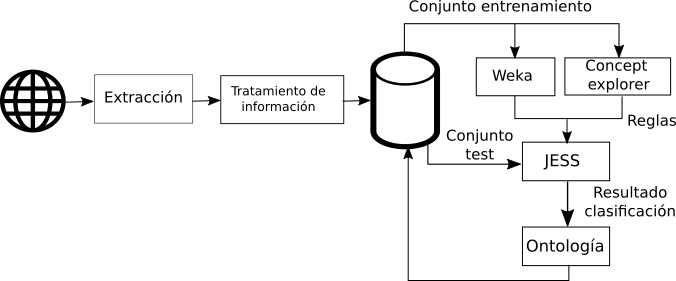
\includegraphics[width=\textwidth]{cron/drawing2.png}
\caption{Infraestructura del sistema}
\end{figure}
\end{center}

La primera tarea es la búsqueda de noticias que no tengamos almacenadas por haber sido publicadas después de la última búsqueda realizada, como el iterar entre los distintos municipios es una operación que requiere tiempo se realizará esta tarea cada 48 horas.

Junto a la tarea anterior debemos ejecutar otra tarea que consideramos una continuación de la anterior, esta es el asignar una categoría a aquellas noticias que hayamos extraído y no tengan una categoría en la web de su municipio y la aplicación de la ontología que hemos creado.

\subsection{Realización de copias de seguridad de la base de datos}

En prevención de un fallo en el gestor de la base de datos u otro fallo del propio servidor, una vez por semana se hará una copia completa de la base de datos para poder recuperar la aplicación en caso de de producirse algún fallo.

\subsection{Eliminación de comentarios considerados negativos}

Una vez cada 24 horas, aquellos comentarios que los usuarios, por votación, consideren negativos serán eliminados si un comentario tiene el número mínimo de votos negativos que consideramos para proceder a su eliminación

\subsection{Corrección de categorías erróneamente asignadas}

De la misma forma que la tarea anterior, una vez al día, se harán correcciones sobre las categorías asignadas a las noticias si un número mínimo de usuarios, a través de la aplicación, marcan que una o varias de las categorías asignadas a una noticia no son correctas.